\subsection{OB-19 (HWB)}
Generátory skutečně náhodných čísel (TRNG), příklad konstrukce, základní vlastnosti. Srovnání s pseudo\-ná\-hod\-ný\-mi generátory (PRNG).


\subsubsection*{PRNG}
\begin{itemize}
	\item Pseudo Random Number Generator
	\item deterministické / algoritmické RNG
	\item má nějaký vnitřní stav a logiku přechodu do dalšího stavu, na základě stavu dává výstup
	\item výhoda je rychlost
	\item jeden z nejznámějších PRNG je lineární kongruenční generátor, definován rekurentním vztahem $X_{n + 1} = (a \cdot X_n + c)$ mod $m$, $X_0$ je počáteční hodnota zvaná seed
	\item $X$ se opakuje nejpozději po $m$ iteracích
	\item kvalita generátoru závisí na vybraných hodnotách $m, a, c$
	\item entropie musí být dodána dobrým seedem
	\item požadované bezpečnostní vlastnosti:
	\begin{itemize}
		\item  musí projít statistickými testy náhodnosti
		\item next-bit test --- na základě předchozích bitů nesmí být následující odhadnutelný
		\item "state compromise" / "backtracking resistance" --- z aktuálního vnitřního stavu generátoru nesmí jít zpětně rekonstruovat předchozí výstupy
	\end{itemize}
\end{itemize}

\subsubsection*{TRNG}
\begin{itemize}
	\item True Random Number Generator
	\item nedeterministický, nepředvídatelný
	\item typicky pomalejší a složitější než PRNG
	\item využívá jako zdroje entropie náhodné fyzikální či jiné procesy, které jsou složité předvídat
	\item horší statistické vlastnosti --- vhodné použít výstup jako seed do PRNG = hybridní RNG
	
	\item příklady: radioaktivní rozpad, teplotní šum, kvantové jevy, nestabilita oscilátoru, chování uživatele, parametry prostředí...
	\item nestabilita oscilátoru: 2 čítače se inkrementují podle 2 oscilátorů, a když jeden čítač dojde na požadovanou hodnotu, z hodnoty druhého se vezmou spodní bity --- náhodné
	\item TRNG založený na SRAM: SRAM po zapnutí napájení má náhodný obsah
	\item pro více bitů entropie lze pustit vícekrát
	\item jako postprocessing lze využít hashovací funkci, nebo např. Von Neumannův dekorelátor:
	
	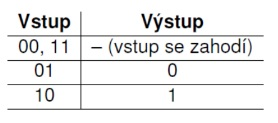
\includegraphics[width=0.4\textwidth]{img/OB-19.jpg}
\end{itemize}